\chapter{تحلیل سرشکن}

\index{amortized analysis@تحلیل سرشکن}

پیچیدگی زمانی یک الگوریتم
اغلب تنها با بررسی ساختار الگوریتم
به‌سادگی تحلیل می‌شود:
الگوریتم شامل چه حلقه‌هایی است
و این حلقه‌ها چند بار اجرا می‌شوند.
با این حال، گاهی اوقات تحلیل مستقیم
تصویر درستی از کارایی الگوریتم ارائه نمی‌دهد.

می‌توان از \key{تحلیل سرشکن} برای تحلیل
الگوریتم‌هایی استفاده کرد که شامل عملیاتی با
پیچیدگی زمانی متغیر هستند.
ایده این است که به جای تمرکز بر تک‌تک عملیات،
کل زمان صرف‌شده برای تمام این عملیات در طول
اجرای الگوریتم برآورد شود.

\section{روش دو اشاره‌گر}

\index{two pointers method@روش دو اشاره‌گر}

در \key{روش دو اشاره‌گر}،
از دو اشاره‌گر برای
پیمایش مقادیر آرایه استفاده می‌شود.
هر دو اشاره‌گر فقط می‌توانند در یک جهت حرکت کنند،
که کارایی الگوریتم را تضمین می‌کند.
سپس به دو مسئله می‌پردازیم که می‌توان با
روش دو اشاره‌گر حل کرد.

\subsubsection{مجموع زیرآرایه}

به عنوان اولین مثال،
مسئله‌ای را در نظر بگیرید که در آن
آرایه‌ای از $n$ عدد صحیح مثبت
و یک مجموع هدف $x$ داده شده است،
و می‌خواهیم زیرآرایه‌ای پیدا کنیم که مجموع آن برابر با $x$ باشد
یا اعلام کنیم چنین زیرآرایه‌ای وجود ندارد.

برای نمونه، آرایه
\begin{center}
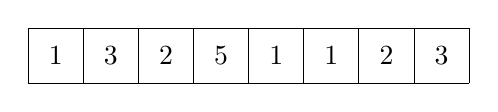
\begin{tikzpicture}[scale=0.7]
\draw (0,0) grid (8,1);

\node at (0.5,0.5) {$1$};
\node at (1.5,0.5) {$3$};
\node at (2.5,0.5) {$2$};
\node at (3.5,0.5) {$5$};
\node at (4.5,0.5) {$1$};
\node at (5.5,0.5) {$1$};
\node at (6.5,0.5) {$2$};
\node at (7.5,0.5) {$3$};
\end{tikzpicture}
\end{center}
شامل زیرآرایه‌ای است که مجموع آن برابر ۸ است:
\begin{center}
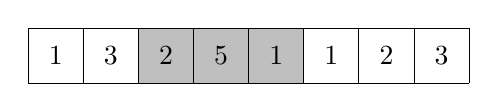
\begin{tikzpicture}[scale=0.7]
\fill[color=lightgray] (2,0) rectangle (5,1);
\draw (0,0) grid (8,1);

\node at (0.5,0.5) {$1$};
\node at (1.5,0.5) {$3$};
\node at (2.5,0.5) {$2$};
\node at (3.5,0.5) {$5$};
\node at (4.5,0.5) {$1$};
\node at (5.5,0.5) {$1$};
\node at (6.5,0.5) {$2$};
\node at (7.5,0.5) {$3$};
\end{tikzpicture}
\end{center}

این مسئله را می‌توان در
زمان $O(n)$ با روش دو اشاره‌گر حل کرد.
ایده کار نگهداری اشاره‌گرهایی است که به
مقدار اول و آخر یک زیرآرایه اشاره می‌کنند.
در هر نوبت، اشاره‌گر چپ یک گام
به راست حرکت می‌کند، و اشاره‌گر راست تا زمانی
که مجموع زیرآرایه حاصل حداکثر $x$ باشد به راست حرکت می‌کند.
اگر مجموع دقیقاً برابر $x$ شود،
جواب پیدا شده است.

به عنوان مثال، آرایه زیر
و مجموع هدف $x=8$ را در نظر بگیرید:
\begin{center}
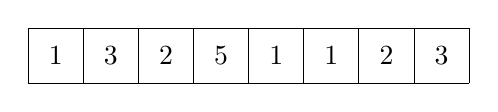
\begin{tikzpicture}[scale=0.7]
\draw (0,0) grid (8,1);

\node at (0.5,0.5) {$1$};
\node at (1.5,0.5) {$3$};
\node at (2.5,0.5) {$2$};
\node at (3.5,0.5) {$5$};
\node at (4.5,0.5) {$1$};
\node at (5.5,0.5) {$1$};
\node at (6.5,0.5) {$2$};
\node at (7.5,0.5) {$3$};
\end{tikzpicture}
\end{center}

زیرآرایه اولیه شامل مقادیر
۱، ۳ و ۲ است که مجموع آن‌ها برابر ۶ می‌شود:

\begin{center}
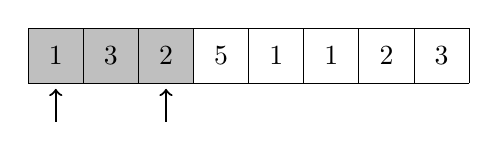
\begin{tikzpicture}[scale=0.7]
\fill[color=lightgray] (0,0) rectangle (3,1);
\draw (0,0) grid (8,1);

\node at (0.5,0.5) {$1$};
\node at (1.5,0.5) {$3$};
\node at (2.5,0.5) {$2$};
\node at (3.5,0.5) {$5$};
\node at (4.5,0.5) {$1$};
\node at (5.5,0.5) {$1$};
\node at (6.5,0.5) {$2$};
\node at (7.5,0.5) {$3$};

\draw[thick,->] (0.5,-0.7) -- (0.5,-0.1);
\draw[thick,->] (2.5,-0.7) -- (2.5,-0.1);
\end{tikzpicture}
\end{center}

سپس اشاره‌گر چپ یک گام به راست می‌رود.
اشاره‌گر راست حرکت نمی‌کند، چون در غیر این صورت
مجموع زیرآرایه از $x$ بیشتر می‌شود.

\begin{center}
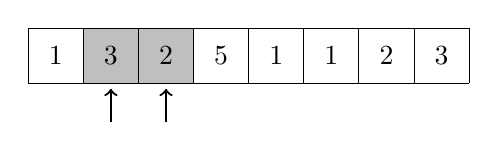
\begin{tikzpicture}[scale=0.7]
\fill[color=lightgray] (1,0) rectangle (3,1);
\draw (0,0) grid (8,1);

\node at (0.5,0.5) {$1$};
\node at (1.5,0.5) {$3$};
\node at (2.5,0.5) {$2$};
\node at (3.5,0.5) {$5$};
\node at (4.5,0.5) {$1$};
\node at (5.5,0.5) {$1$};
\node at (6.5,0.5) {$2$};
\node at (7.5,0.5) {$3$};

\draw[thick,->] (1.5,-0.7) -- (1.5,-0.1);
\draw[thick,->] (2.5,-0.7) -- (2.5,-0.1);
\end{tikzpicture}
\end{center}

مجدداً اشاره‌گر چپ یک گام به راست حرکت می‌کند،
و این بار اشاره‌گر راست سه گام
به راست می‌رود.
مجموع زیرآرایه $2+5+1=8$ است، بنابراین زیرآرایه‌ای
با مجموع $x$ پیدا شده است.

\begin{center}
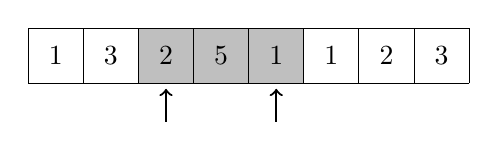
\begin{tikzpicture}[scale=0.7]
\fill[color=lightgray] (2,0) rectangle (5,1);
\draw (0,0) grid (8,1);

\node at (0.5,0.5) {$1$};
\node at (1.5,0.5) {$3$};
\node at (2.5,0.5) {$2$};
\node at (3.5,0.5) {$5$};
\node at (4.5,0.5) {$1$};
\node at (5.5,0.5) {$1$};
\node at (6.5,0.5) {$2$};
\node at (7.5,0.5) {$3$};

\draw[thick,->] (2.5,-0.7) -- (2.5,-0.1);
\draw[thick,->] (4.5,-0.7) -- (4.5,-0.1);
\end{tikzpicture}
\end{center}

زمان اجرای الگوریتم به تعداد گام‌های
حرکت اشاره‌گر راست وابسته است.
گرچه کران بالای مفیدی برای تعداد گام‌های حرکت اشاره‌گر
در یک نوبت \emph{تک} وجود ندارد،
می‌دانیم اشاره‌گر \emph{در مجموع}
$O(n)$ گام در طول الگوریتم حرکت می‌کند،
زیرا فقط به سمت راست می‌رود.

از آنجا که هر دو اشاره‌گر چپ و راست
در طول الگوریتم $O(n)$ گام حرکت می‌کنند،
الگوریتم در زمان $O(n)$ اجرا می‌شود.

\subsubsection{مسئله 2SUM}

\index{مسئله 2SUM}

مسئله دیگری که با روش دو اشاره‌گر
حل می‌شود مسئله زیر است،
که با نام \key{مسئله 2SUM} نیز شناخته می‌شود:
با فرض یک آرایه شامل $n$ عدد و
مجموع هدف $x$، دو مقدار
از آرایه بیابید که مجموع آن‌ها $x$ شود،
یا اعلام کنید چنین مقادیری وجود ندارند.

برای حل مسئله، ابتدا
مقادیر آرایه را به ترتیب صعودی مرتب می‌کنیم.
پس از آن، با استفاده از دو اشاره‌گر
روی آرایه پیمایش می‌کنیم.
اشاره‌گر چپ از مقدار نخست آغاز شده
و در هر نوبت یک گام به راست می‌رود.
اشاره‌گر راست از مقدار آخر شروع شده
و تا زمانی که مجموع مقادیر
چپ و راست حداکثر برابر $x$ شود به چپ می‌رود.
اگر مجموع دقیقاً $x$ باشد،
پاسخ پیدا شده است.

برای نمونه، آرایه زیر
و مجموع هدف $x=12$ را در نظر بگیرید:
\begin{center}
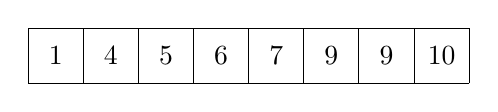
\begin{tikzpicture}[scale=0.7]
\draw (0,0) grid (8,1);

\node at (0.5,0.5) {$1$};
\node at (1.5,0.5) {$4$};
\node at (2.5,0.5) {$5$};
\node at (3.5,0.5) {$6$};
\node at (4.5,0.5) {$7$};
\node at (5.5,0.5) {$9$};
\node at (6.5,0.5) {$9$};
\node at (7.5,0.5) {$10$};
\end{tikzpicture}
\end{center}

موقعیت اولیه اشاره‌گرها
به شکل زیر است.
مجموع مقادیر $1+10=11$ است
که از $x$ کوچک‌تر است.

\begin{center}
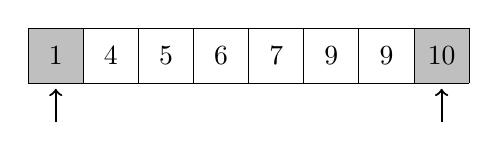
\begin{tikzpicture}[scale=0.7]
\fill[color=lightgray] (0,0) rectangle (1,1);
\fill[color=lightgray] (7,0) rectangle (8,1);
\draw (0,0) grid (8,1);

\node at (0.5,0.5) {$1$};
\node at (1.5,0.5) {$4$};
\node at (2.5,0.5) {$5$};
\node at (3.5,0.5) {$6$};
\node at (4.5,0.5) {$7$};
\node at (5.5,0.5) {$9$};
\node at (6.5,0.5) {$9$};
\node at (7.5,0.5) {$10$};

\draw[thick,->] (0.5,-0.7) -- (0.5,-0.1);
\draw[thick,->] (7.5,-0.7) -- (7.5,-0.1);
\end{tikzpicture}
\end{center}

سپس اشاره‌گر چپ یک گام به راست می‌رود.
اشاره‌گر راست سه گام به چپ حرکت می‌کند
و مجموع برابر با $4+7=11$ می‌شود.

\begin{center}
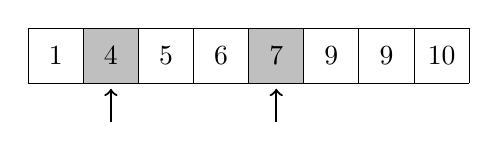
\begin{tikzpicture}[scale=0.7]
\fill[color=lightgray] (1,0) rectangle (2,1);
\fill[color=lightgray] (4,0) rectangle (5,1);
\draw (0,0) grid (8,1);

\node at (0.5,0.5) {$1$};
\node at (1.5,0.5) {$4$};
\node at (2.5,0.5) {$5$};
\node at (3.5,0.5) {$6$};
\node at (4.5,0.5) {$7$};
\node at (5.5,0.5) {$9$};
\node at (6.5,0.5) {$9$};
\node at (7.5,0.5) {$10$};

\draw[thick,->] (1.5,-0.7) -- (1.5,-0.1);
\draw[thick,->] (4.5,-0.7) -- (4.5,-0.1);
\end{tikzpicture}
\end{center}

پس از این، اشاره‌گر چپ دوباره یک گام به راست می‌رود.
اشاره‌گر راست حرکت نمی‌کند و جواب
$5+7=12$ پیدا می‌شود.

\begin{center}
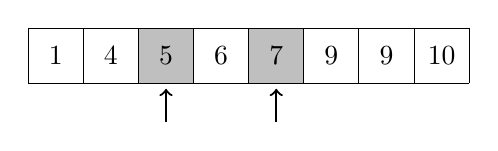
\begin{tikzpicture}[scale=0.7]
\fill[color=lightgray] (2,0) rectangle (3,1);
\fill[color=lightgray] (4,0) rectangle (5,1);
\draw (0,0) grid (8,1);

\node at (0.5,0.5) {$1$};
\node at (1.5,0.5) {$4$};
\node at (2.5,0.5) {$5$};
\node at (3.5,0.5) {$6$};
\node at (4.5,0.5) {$7$};
\node at (5.5,0.5) {$9$};
\node at (6.5,0.5) {$9$};
\node at (7.5,0.5) {$10$};

\draw[thick,->] (2.5,-0.7) -- (2.5,-0.1);
\draw[thick,->] (4.5,-0.7) -- (4.5,-0.1);
\end{tikzpicture}
\end{center}

زمان اجرای الگوریتم
$O(n \log n)$ است، زیرا ابتدا
آرایه در زمان $O(n \log n)$ مرتب شده
و سپس هر دو اشاره‌گر $O(n)$ گام جابه‌جا می‌شوند.

توجه کنید حل مسئله
به روش دیگر در زمان $O(n \log n)$ با جستجوی دودویی نیز ممکن است.
در این روش، روی آرایه پیمایش کرده
و به ازای هر مقدار آرایه، تلاش می‌کنیم مقدار دیگر
سازنده مجموع $x$ را بیابیم.
این کار با انجام $n$ جستجوی دودویی ممکن است
که هر کدام $O(\log n)$ زمان می‌برد.

\index{مسئله 3SUM}
مسئله دشوارتر، \key{مسئله 3SUM} است که یافتن \emph{سه} مقدار از آرایه با مجموع $x$ را می‌خواهد.
با ایده الگوریتم بالا، این مسئله در زمان $O(n^2)$ حل می‌شود\footnote{مدت‌ها گمان می‌رفت حل مسئله 3SUM سریع‌تر از زمان $O(n^2)$ ممکن نیست.
اما در سال ۲۰۱۴ مشخص شد \cite{gro14} که چنین نیست.}.
روش آن را می‌دانید؟

\section{نزدیک‌ترین عناصر کوچک‌تر}

\index{نزدیک‌ترین عناصر کوچک‌تر}

تحلیل سرشکن اغلب برای تخمین تعداد عملیات انجام‌شده روی ساختمان داده به کار می‌رود.
عملیات ممکن است نامتوازن توزیع شوند؛ به طوری که بیشتر عملیات در فاز خاصی از الگوریتم رخ دهند، اما تعداد کل عملیات محدود است.

به عنوان مثال، مسئله یافتن \key{نزدیک‌ترین عنصر کوچک‌تر} برای هر عنصر آرایه را در نظر بگیرید؛ یعنی اولین عنصر کوچک‌تر پیش از آن در آرایه.
ممکن است چنین عنصری وجود نداشته باشد که در این حالت الگوریتم باید این را گزارش کند.
در ادامه روش حل کارآمد مسئله با ساختار پشته بررسی می‌شود.

آرایه را از چپ به راست پیمایش کرده و پشته‌ای از عناصر آرایه نگه می‌داریم.
در هر موقعیت آرایه، عناصر پشته را تا جایی حذف می‌کنیم که عنصر بالای پشته کوچک‌تر از عنصر فعلی شود یا پشته خالی گردد.
سپس گزارش می‌دهیم عنصر بالای پشته نزدیک‌ترین عنصر کوچک‌تر به عنصر فعلی است؛ اگر پشته خالی باشد، چنین عنصری وجود ندارد.
در نهایت، عنصر فعلی را به پشته اضافه می‌کنیم.

به عنوان مثال، آرایه زیر را در نظر بگیرید:
\begin{center}
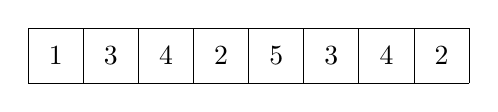
\begin{tikzpicture}[scale=0.7]
\draw (0,0) grid (8,1);

\node at (0.5,0.5) {$1$};
\node at (1.5,0.5) {$3$};
\node at (2.5,0.5) {$4$};
\node at (3.5,0.5) {$2$};
\node at (4.5,0.5) {$5$};
\node at (5.5,0.5) {$3$};
\node at (6.5,0.5) {$4$};
\node at (7.5,0.5) {$2$};
\end{tikzpicture}
\end{center}

ابتدا عناصر ۱، ۳ و ۴ به پشته اضافه می‌شوند، زیرا هر عنصر بزرگ‌تر از عنصر قبلی است.
بنابراین نزدیک‌ترین عنصر کوچک‌تر به ۴ برابر ۳، و نزدیک‌ترین عنصر کوچک‌تر به ۳ برابر ۱ است.
\begin{center}
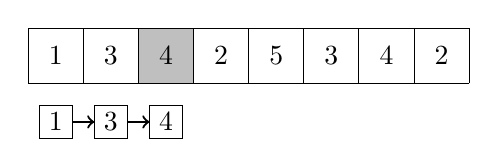
\begin{tikzpicture}[scale=0.7]
\fill[color=lightgray] (2,0) rectangle (3,1);
\draw (0,0) grid (8,1);

\node at (0.5,0.5) {$1$};
\node at (1.5,0.5) {$3$};
\node at (2.5,0.5) {$4$};
\node at (3.5,0.5) {$2$};
\node at (4.5,0.5) {$5$};
\node at (5.5,0.5) {$3$};
\node at (6.5,0.5) {$4$};
\node at (7.5,0.5) {$2$};

\draw (0.2,0.2-1.2) rectangle (0.8,0.8-1.2);
\draw (1.2,0.2-1.2) rectangle (1.8,0.8-1.2);
\draw (2.2,0.2-1.2) rectangle (2.8,0.8-1.2);

\node at (0.5,0.5-1.2) {$1$};
\node at (1.5,0.5-1.2) {$3$};
\node at (2.5,0.5-1.2) {$4$};

\draw[->,thick] (0.8,0.5-1.2) -- (1.2,0.5-1.2);
\draw[->,thick] (1.8,0.5-1.2) -- (2.2,0.5-1.2);
\end{tikzpicture}
\end{center}

عنصر بعدی ۲ از دو عنصر بالای پشته کوچک‌تر است.
بنابراین، عناصر ۳ و ۴ از پشته حذف می‌شوند و سپس عنصر ۲ به پشته اضافه می‌شود.
نزدیک‌ترین عنصر کوچک‌تر به آن ۱ است:
\begin{center}
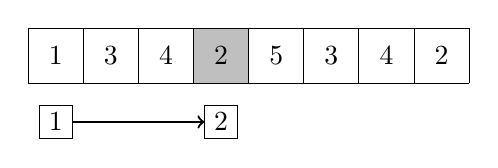
\begin{tikzpicture}[scale=0.7]
\fill[color=lightgray] (3,0) rectangle (4,1);
\draw (0,0) grid (8,1);

\node at (0.5,0.5) {$1$};
\node at (1.5,0.5) {$3$};
\node at (2.5,0.5) {$4$};
\node at (3.5,0.5) {$2$};
\node at (4.5,0.5) {$5$};
\node at (5.5,0.5) {$3$};
\node at (6.5,0.5) {$4$};
\node at (7.5,0.5) {$2$};

\draw (0.2,0.2-1.2) rectangle (0.8,0.8-1.2);
\draw (3.2,0.2-1.2) rectangle (3.8,0.8-1.2);

\node at (0.5,0.5-1.2) {$1$};
\node at (3.5,0.5-1.2) {$2$};

\draw[->,thick] (0.8,0.5-1.2) -- (3.2,0.5-1.2);
\end{tikzpicture}
\end{center}

سپس، عنصر ۵ از عنصر ۲ بزرگ‌تر است،
پس به پشته اضافه می‌شود و نزدیک‌ترین عنصر کوچک‌تر به آن ۲ است:
\begin{center}
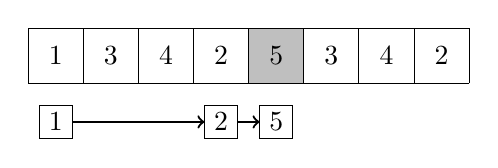
\begin{tikzpicture}[scale=0.7]
\fill[color=lightgray] (4,0) rectangle (5,1);
\draw (0,0) grid (8,1);

\node at (0.5,0.5) {$1$};
\node at (1.5,0.5) {$3$};
\node at (2.5,0.5) {$4$};
\node at (3.5,0.5) {$2$};
\node at (4.5,0.5) {$5$};
\node at (5.5,0.5) {$3$};
\node at (6.5,0.5) {$4$};
\node at (7.5,0.5) {$2$};

\draw (0.2,0.2-1.2) rectangle (0.8,0.8-1.2);
\draw (3.2,0.2-1.2) rectangle (3.8,0.8-1.2);
\draw (4.2,0.2-1.2) rectangle (4.8,0.8-1.2);

\node at (0.5,0.5-1.2) {$1$};
\node at (3.5,0.5-1.2) {$2$};
\node at (4.5,0.5-1.2) {$5$};

\draw[->,thick] (0.8,0.5-1.2) -- (3.2,0.5-1.2);
\draw[->,thick] (3.8,0.5-1.2) -- (4.2,0.5-1.2);
\end{tikzpicture}
\end{center}

پس از این، عنصر ۵ از پشته حذف می‌شود
و عناصر ۳ و ۴ به پشته اضافه می‌شوند:
\begin{center}
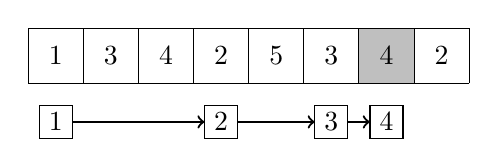
\begin{tikzpicture}[scale=0.7]
\fill[color=lightgray] (6,0) rectangle (7,1);
\draw (0,0) grid (8,1);

\node at (0.5,0.5) {$1$};
\node at (1.5,0.5) {$3$};
\node at (2.5,0.5) {$4$};
\node at (3.5,0.5) {$2$};
\node at (4.5,0.5) {$5$};
\node at (5.5,0.5) {$3$};
\node at (6.5,0.5) {$4$};
\node at (7.5,0.5) {$2$};

\draw (0.2,0.2-1.2) rectangle (0.8,0.8-1.2);
\draw (3.2,0.2-1.2) rectangle (3.8,0.8-1.2);
\draw (5.2,0.2-1.2) rectangle (5.8,0.8-1.2);
\draw (6.2,0.2-1.2) rectangle (6.8,0.8-1.2);

\node at (0.5,0.5-1.2) {$1$};
\node at (3.5,0.5-1.2) {$2$};
\node at (5.5,0.5-1.2) {$3$};
\node at (6.5,0.5-1.2) {$4$};

\draw[->,thick] (0.8,0.5-1.2) -- (3.2,0.5-1.2);
\draw[->,thick] (3.8,0.5-1.2) -- (5.2,0.5-1.2);
\draw[->,thick] (5.8,0.5-1.2) -- (6.2,0.5-1.2);
\end{tikzpicture}
\end{center}

در نهایت، همه عناصر به جز ۱ از پشته حذف می‌شوند
و آخرین عنصر ۲ به پشته اضافه می‌شود:

\begin{center}
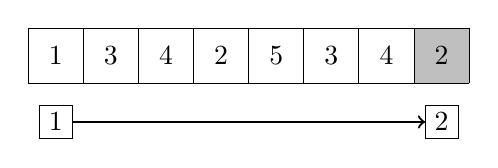
\begin{tikzpicture}[scale=0.7]
\fill[color=lightgray] (7,0) rectangle (8,1);
\draw (0,0) grid (8,1);

\node at (0.5,0.5) {$1$};
\node at (1.5,0.5) {$3$};
\node at (2.5,0.5) {$4$};
\node at (3.5,0.5) {$2$};
\node at (4.5,0.5) {$5$};
\node at (5.5,0.5) {$3$};
\node at (6.5,0.5) {$4$};
\node at (7.5,0.5) {$2$};

\draw (0.2,0.2-1.2) rectangle (0.8,0.8-1.2);
\draw (7.2,0.2-1.2) rectangle (7.8,0.8-1.2);

\node at (0.5,0.5-1.2) {$1$};
\node at (7.5,0.5-1.2) {$2$};

\draw[->,thick] (0.8,0.5-1.2) -- (7.2,0.5-1.2);
\end{tikzpicture}
\end{center}

کارایی الگوریتم به تعداد کل عملیات‌های پشته وابسته است.
اگر عنصر کنونی بزرگ‌تر از عنصر بالای پشته باشد،
مستقیماً به پشته اضافه می‌شود که کارآمد است.
با این حال، گاهی پشته شامل چندین عنصر بزرگ‌تر است
و حذف آن‌ها زمان می‌برد.
با این وجود، هر عنصر \emph{دقیقاً یک بار} به پشته اضافه می‌شود
و \emph{حداکثر یک بار} از پشته حذف می‌گردد.
بنابراین، هر عنصر موجب $O(1)$ عملیات پشته می‌شود
و الگوریتم در زمان $O(n)$ اجرا می‌شود.

\section{کمینه در پنجره لغزان}

\index{پنجره لغزان}
\index{کمینه در پنجره لغزان}

یک \key{پنجره لغزان} زیرآرایه‌ای با اندازه ثابت است
که از چپ به راست روی آرایه حرکت می‌کند.
در هر موقعیت پنجره،
می‌خواهیم اطلاعاتی درباره عناصر درون پنجره محاسبه کنیم.
در این بخش، تمرکز روی مسئله نگهداری
\key{کمینه در پنجره لغزان} است،
به این معنی که باید کوچک‌ترین مقدار درون هر پنجره را گزارش کنیم.

کمینه در پنجره لغزان را می‌توان با ایده‌ای مشابه
محاسبه نزدیک‌ترین عناصر کوچک‌تر به دست آورد.
یک صف نگهداری می‌کنیم که در آن هر عنصر از عنصر قبلی بزرگ‌تر است،
و عنصر اول همیشه متناظر با کمینه عنصر درون پنجره است.
پس از هر حرکت پنجره،
عناصر را از انتهای صف حذف می‌کنیم
تا زمانی که آخرین عنصر صف از عنصر جدید پنجره کوچک‌تر شود،
یا صف خالی گردد.
همچنین اگر عنصر اول صف دیگر درون پنجره نباشد،
آن را حذف می‌کنیم.
در نهایت، عنصر جدید پنجره را به انتهای صف اضافه می‌کنیم.

به عنوان مثال، آرایه زیر را در نظر بگیرید:

\begin{center}
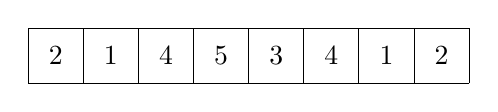
\begin{tikzpicture}[scale=0.7]
\draw (0,0) grid (8,1);

\node at (0.5,0.5) {$2$};
\node at (1.5,0.5) {$1$};
\node at (2.5,0.5) {$4$};
\node at (3.5,0.5) {$5$};
\node at (4.5,0.5) {$3$};
\node at (5.5,0.5) {$4$};
\node at (6.5,0.5) {$1$};
\node at (7.5,0.5) {$2$};
\end{tikzpicture}
\end{center}

فرض کنید اندازه پنجره لغزان برابر ۴ است.
در موقعیت اول پنجره، کوچک‌ترین مقدار ۱ است:
\begin{center}
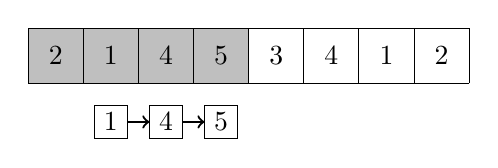
\begin{tikzpicture}[scale=0.7]
\fill[color=lightgray] (0,0) rectangle (4,1);
\draw (0,0) grid (8,1);

\node at (0.5,0.5) {$2$};
\node at (1.5,0.5) {$1$};
\node at (2.5,0.5) {$4$};
\node at (3.5,0.5) {$5$};
\node at (4.5,0.5) {$3$};
\node at (5.5,0.5) {$4$};
\node at (6.5,0.5) {$1$};
\node at (7.5,0.5) {$2$};

\draw (1.2,0.2-1.2) rectangle (1.8,0.8-1.2);
\draw (2.2,0.2-1.2) rectangle (2.8,0.8-1.2);
\draw (3.2,0.2-1.2) rectangle (3.8,0.8-1.2);

\node at (1.5,0.5-1.2) {$1$};
\node at (2.5,0.5-1.2) {$4$};
\node at (3.5,0.5-1.2) {$5$};

\draw[->,thick] (1.8,0.5-1.2) -- (2.2,0.5-1.2);
\draw[->,thick] (2.8,0.5-1.2) -- (3.2,0.5-1.2);
\end{tikzpicture}
\end{center}

سپس پنجره یک گام به راست حرکت می‌کند.
عنصر جدید ۳ از عناصر ۴ و ۵ داخل صف کوچک‌تر است، بنابراین عناصر ۴ و ۵ از صف حذف می‌شوند
و عنصر ۳ به صف اضافه می‌شود.
کوچک‌ترین مقدار همچنان ۱ است.
\begin{center}
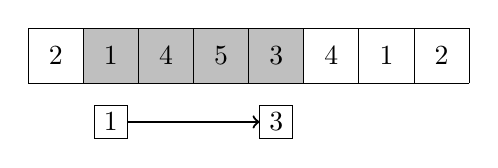
\begin{tikzpicture}[scale=0.7]
\fill[color=lightgray] (1,0) rectangle (5,1);
\draw (0,0) grid (8,1);

\node at (0.5,0.5) {$2$};
\node at (1.5,0.5) {$1$};
\node at (2.5,0.5) {$4$};
\node at (3.5,0.5) {$5$};
\node at (4.5,0.5) {$3$};
\node at (5.5,0.5) {$4$};
\node at (6.5,0.5) {$1$};
\node at (7.5,0.5) {$2$};

\draw (1.2,0.2-1.2) rectangle (1.8,0.8-1.2);
\draw (4.2,0.2-1.2) rectangle (4.8,0.8-1.2);

\node at (1.5,0.5-1.2) {$1$};
\node at (4.5,0.5-1.2) {$3$};

\draw[->,thick] (1.8,0.5-1.2) -- (4.2,0.5-1.2);
\end{tikzpicture}
\end{center}

پس از این، پنجره دوباره حرکت می‌کند
و کوچک‌ترین عنصر یعنی ۱
دیگر به پنجره تعلق ندارد.
بنابراین، از صف حذف می‌شود و کوچک‌ترین مقدار اکنون ۳ است. همچنین عنصر جدید ۴ به صف افزوده می‌شود.
\begin{center}
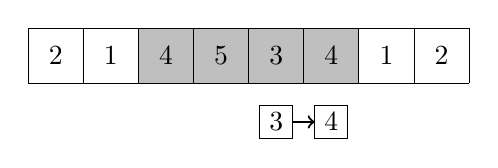
\begin{tikzpicture}[scale=0.7]
\fill[color=lightgray] (2,0) rectangle (6,1);
\draw (0,0) grid (8,1);

\node at (0.5,0.5) {$2$};
\node at (1.5,0.5) {$1$};
\node at (2.5,0.5) {$4$};
\node at (3.5,0.5) {$5$};
\node at (4.5,0.5) {$3$};
\node at (5.5,0.5) {$4$};
\node at (6.5,0.5) {$1$};
\node at (7.5,0.5) {$2$};

\draw (4.2,0.2-1.2) rectangle (4.8,0.8-1.2);
\draw (5.2,0.2-1.2) rectangle (5.8,0.8-1.2);

\node at (4.5,0.5-1.2) {$3$};
\node at (5.5,0.5-1.2) {$4$};

\draw[->,thick] (4.8,0.5-1.2) -- (5.2,0.5-1.2);
\end{tikzpicture}
\end{center}

عنصر جدید بعدی ۱ از تمام عناصر صف کوچک‌تر است.
بنابراین، تمام عناصر از صف حذف می‌شوند
و صف تنها شامل عنصر ۱ خواهد بود:
\begin{center}
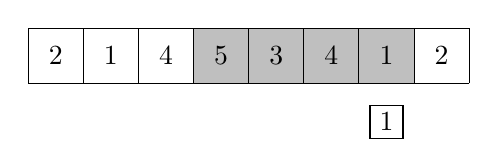
\begin{tikzpicture}[scale=0.7]
\fill[color=lightgray] (3,0) rectangle (7,1);
\draw (0,0) grid (8,1);

\node at (0.5,0.5) {$2$};
\node at (1.5,0.5) {$1$};
\node at (2.5,0.5) {$4$};
\node at (3.5,0.5) {$5$};
\node at (4.5,0.5) {$3$};
\node at (5.5,0.5) {$4$};
\node at (6.5,0.5) {$1$};
\node at (7.5,0.5) {$2$};

\draw (6.2,0.2-1.2) rectangle (6.8,0.8-1.2);

\node at (6.5,0.5-1.2) {$1$};
\end{tikzpicture}
\end{center}

در نهایت پنجره به آخرین موقعیت خود می‌رسد.
عنصر ۲ به صف اضافه می‌شود،
اما کوچک‌ترین مقدار درون پنجره
همچنان ۱ است.
\begin{center}
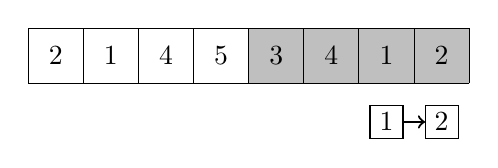
\begin{tikzpicture}[scale=0.7]
\fill[color=lightgray] (4,0) rectangle (8,1);
\draw (0,0) grid (8,1);

\node at (0.5,0.5) {$2$};
\node at (1.5,0.5) {$1$};
\node at (2.5,0.5) {$4$};
\node at (3.5,0.5) {$5$};
\node at (4.5,0.5) {$3$};
\node at (5.5,0.5) {$4$};
\node at (6.5,0.5) {$1$};
\node at (7.5,0.5) {$2$};

\draw (6.2,0.2-1.2) rectangle (6.8,0.8-1.2);
\draw (7.2,0.2-1.2) rectangle (7.8,0.8-1.2);

\node at (6.5,0.5-1.2) {$1$};
\node at (7.5,0.5-1.2) {$2$};

\draw[->,thick] (6.8,0.5-1.2) -- (7.2,0.5-1.2);
\end{tikzpicture}
\end{center}

از آنجا که هر عنصر آرایه
دقیقاً یک بار به صف اضافه می‌شود و
حداکثر یک بار از صف حذف می‌گردد،
این الگوریتم در زمان $O(n)$ عمل می‌کند.